\subsection*{Wireless Channel}
Le but est de définir le canal sans fil avec plus de précision que le modèle AWGN et de donner un
plan de référence plus réaliste pour les systèmes de communication.

\textbf{Fading lent:}

sont des modèles basés sur la puissance du signal en fonction
de la distance.

\underline{Open sky attenuation}

Friis: $P_r=P_t G_r G_t\left(\frac{\lambda}{4\pi d}\right)^2[W]$ avec $\lambda=\frac{C}{f}[m]$

Atténuation: $Att=\left(\frac{4\pi d}{\lambda}\right)^2$ Il faut prendre la vitesse de la lumière à $C=300 000$

Friis en dB: $P_r|_{dBm}=P_t|_{dBm}+G_r|_{dBi}+G_t|_{dBi}+20\log_{10}(\lambda)-20\log_{10}(4\pi d)$
Pour une antenne omnidirectionnelle $G_r|_{dBi}=G_t|_{dBi}=0$

Friis avec obstacle: $P_r=P_t G_r G_t\frac{\lambda^2}{(4\pi)^2 d\gamma}$
avec $\gamma$ le coefficient de propagation qui dépend de l'environnement:

\begin{tabular}{l|l}
    Environment                        & $\gamma$   \\ \hline
    Free space:                        & 2          \\
    Urban area cellular radio:         & 2.7 to 3.5 \\
    Shadowed urban cellular radio:     & 3 to 5     \\
    Inside a building - line of sight: & 1.6 to 1.8 \\
    Obstructed in building:            & 4 to 6     \\
    Obstructed in factory:             & 2 to 3
\end{tabular}

\underline{Shannon with fading}:

La capacité du canal: $C_{fading}=B\log_2(1+\frac{S}{N}|h|^2)$ avec $h$ le fading un nombre complexe

Comme $h$ est une variable aléatoire, on utilise la moyenne statistique:
$C_{fading}=E[B\log_2(1+\frac{S}{N}|h|^2)]$

\underline{Log-distance model}: $P_r=P_t\cdot\text{Att}_{d_0}(\frac{d_0}{d})^\gamma X_g$
C'est une amélioration du modèle de Friis qui prend en l'aléatoire du canal. Basé sur une atténuation
à $d_0$ et un coefficient $\gamma$ qui dépend de l'environnement. $X_g$ variable aléatoire qui
qui correspond au fading.

\underline{Ground reflection model}:

\begin{figure}[H]
    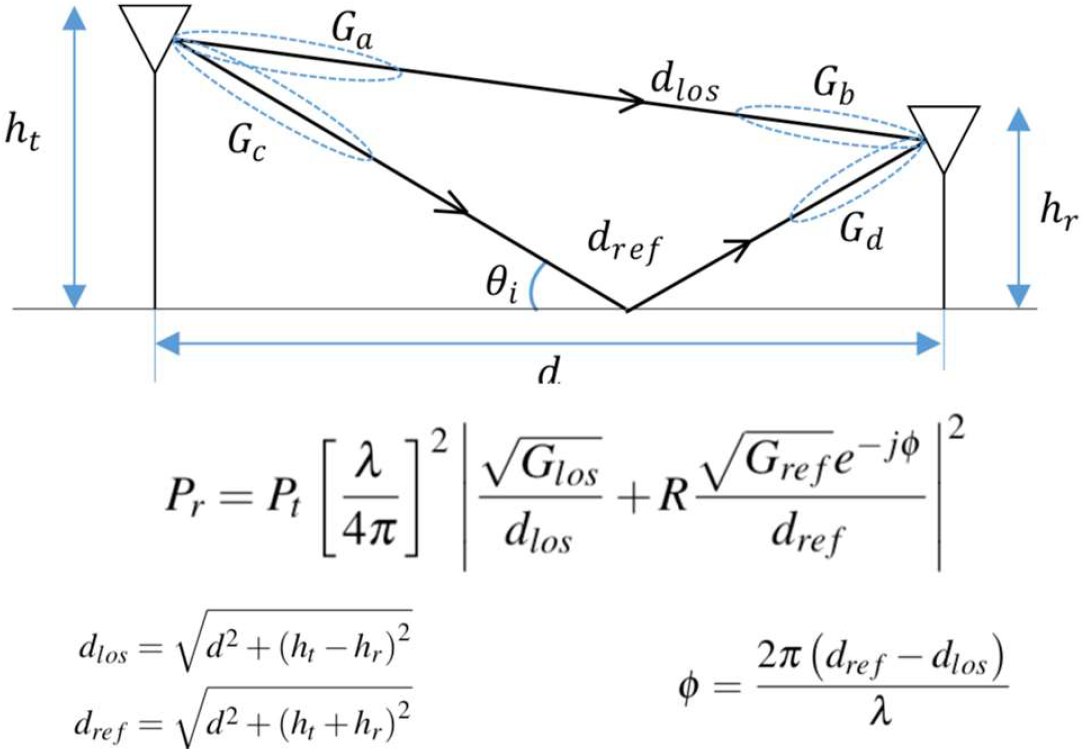
\includegraphics[width=\linewidth]{images/ground_reflection_model.png}
\end{figure}

\underline{Fresnel zone}: $R=\frac{1}{2}\sqrt{\frac{cD}{f}}$ avec D la distance entre les antennes.
C'est une sorte de globe elliptique qui entoure la ligne de visée.

\textbf{Fading rapide:}

sont des modèles basés sur la distribution statistique de l'amplitude
du signal en fonction des réflexions multiples.

\underline{Rayleigh distribution}: $p(x)=\frac{x}{\sigma^2}e^{-\frac{x^2}{2\sigma^2}}$ avec $x$
l'amplitude du signal et $\sigma$ l'écart type.

\underline{Rice distribution}: $p(x)=\frac{x}{\sigma^2}e^{-\frac{x^2+k^2}{2\sigma^2}}I_0\left(\frac{kx}{\sigma^2}\right)$
avec $k$ le facteur de K et $I_0$ la fonction de Bessel modifiée d'ordre 0.

\underline{Nakagami distribution}: $p(x)=\frac{2m^m}{\Gamma(m)\Omega^m}x^{2m-1}e^{-\frac{m}{\Omega}x^2}$
avec $m$ le facteur de Nakagami et $\Omega$ le facteur de fading.

